% answers.tex —— 2019 年·北京卷·理科 · 参考答案与详细解析片段
% 由 tools/generate_projects.py 依来源总账自 2019/2019_数学真题_北京卷理_试题.md + 2019/2019_数学真题_北京卷理_解析正文.md + 2019/2019_数学真题_北京卷理_答案要点.md 生成，勿手改（改源 MD 后重跑）

\begin{gktip}
固定源没有答案页；以下为非官方推导，不能称为官方答案。
\end{gktip}

\gkpart{一、选择题}

\begin{answer}
\gksolhead{1}{}

\textbf{题目}：

已知复数 $z = 2 + \mathrm{i}$, 则 $z \cdot \bar{z} =$（ ）。

(A) $\sqrt{3}$　(B) $\sqrt{5}$　(C) $3$　(D) $5$

\Needspace{4\baselineskip}
\textbf{解析}

已知复数 $z = 2 + \mathrm{i}$，则其共轭复数为 $\bar{z} = 2 - \mathrm{i}$。
\Needspace{5\baselineskip}
计算复数与其共轭复数的乘积：
\nopagebreak[4]
\[z \cdot \bar{z} = (2 + \mathrm{i})(2 - \mathrm{i}) = 2^2 - \mathrm{i}^2 = 4 - (-1) = 5.\]
故选 \textbf{D}。

\gkanswer{答案：D}

\end{answer}
\begin{answer}
\gksolhead{2}{}

\textbf{题目}：

执行如图所示的程序框图, 输出的 $s$ 值为（ ）。
\nopagebreak[4]
\begin{center}\begin{tikzpicture}[>=latex, font=\small, scale=0.9]
  \tikzstyle{startstop} = [draw, rounded corners=8pt, minimum width=1.8cm, minimum height=0.65cm, text centered]
  \tikzstyle{io} = [draw, trapezium, trapezium left angle=70, trapezium right angle=110, minimum width=1.8cm, minimum height=0.65cm, text centered]
  \tikzstyle{process} = [draw, minimum width=2.0cm, minimum height=0.65cm, text centered]
  \tikzstyle{decision} = [draw, diamond, aspect=2, minimum width=2.2cm, minimum height=0.75cm, text centered]
  \tikzstyle{arrow} = [thick, ->]

  \node (start) [startstop] at (0, 0) {开始};
  \node (init) [process] at (0, -1.0) {$k = 1,\ s = 1$};
  \node (proc) [process] at (0, -2.2) {$s = \dfrac{2s}{3s - 2}$};
  \node (dec) [decision] at (0, -3.5) {$k \geqslant 3$?};
  \node (out) [io] at (0, -4.8) {输出 $s$};
  \node (stop) [startstop] at (0, -5.7) {结束};
  \node (inc) [process] at (2.2, -2.85) {$k = k + 1$};

  \draw[arrow] (start) -- (init);
  \draw[arrow] (init) -- (proc);
  \draw[arrow] (proc) -- (dec);
  \draw[arrow] (dec) -- node[right] {是} (out);
  \draw[arrow] (out) -- (stop);

  \draw[arrow] (dec.east) -| node[above, pos=0.25] {否} (inc.south);
  \draw[arrow] (inc.north) |- ([yshift=0.3cm]proc.north);
\end{tikzpicture}
\end{center}
\nopagebreak[4]
(A) $1$　(B) $2$　(C) $3$　(D) $4$

\Needspace{4\baselineskip}
\textbf{解析}

根据程序框图逐步执行：
\begin{itemize}
\item 初始状态：$k = 1, s = 1$；
\item 第 1 次计算：
\end{itemize}
\nopagebreak[4]
\[s = \frac{2s}{3s - 2} = \frac{2 \times 1}{3 \times 1 - 2} = \frac{2}{1} = 2.\]
  判断 $k \geqslant 3$（即 $1 \geqslant 3$）为“否”，执行 $k = k + 1 = 2$；
\begin{itemize}
\item 第 2 次计算：
\end{itemize}
\nopagebreak[4]
\[s = \frac{2 \times 2}{3 \times 2 - 2} = \frac{4}{4} = 1.\]
  判断 $k \geqslant 3$（即 $2 \geqslant 3$）为“否”，执行 $k = k + 1 = 3$；
\begin{itemize}
\item 第 3 次计算：
\end{itemize}
\nopagebreak[4]
\[s = \frac{2 \times 1}{3 \times 1 - 2} = 2.\]
  判断 $k \geqslant 3$（即 $3 \geqslant 3$）为“是”，退出循环。
输出 $s$ 的值为 2。
故选 \textbf{B}。

\gkanswer{答案：B}

\end{answer}
\begin{answer}
\gksolhead{3}{}

\textbf{题目}：

已知直线 $l$ 的参数方程为 $\begin{cases} x = 1 + 3t, \\ y = 2 + 4t \end{cases}$（$t$ 为参数）, 则点 $(1, 0)$ 到直线 $l$ 的距离是（ ）。

(A) $\dfrac{1}{5}$　(B) $\dfrac{2}{5}$　(C) $\dfrac{4}{5}$　(D) $\dfrac{6}{5}$

\Needspace{4\baselineskip}
\textbf{解析}

将直线 $l$ 的参数方程 $\begin{cases} x = 1 + 3t \\ y = 2 + 4t \end{cases}$ 化为一般方程：
\Needspace{5\baselineskip}
由第一式得 $t = \dfrac{x - 1}{3}$，代入第二式得：
\nopagebreak[4]
\[y = 2 + 4 \cdot \frac{x - 1}{3} \implies 3y = 6 + 4x - 4 \implies 4x - 3y + 2 = 0.\]
\Needspace{5\baselineskip}
根据点到直线的距离公式，点 $(1, 0)$ 到直线 $4x - 3y + 2 = 0$ 的距离为：
\nopagebreak[4]
\[d = \frac{|4 \times 1 - 3 \times 0 + 2|}{\sqrt{4^2 + (-3)^2}} = \frac{|6|}{\sqrt{16 + 9}} = \frac{6}{5}.\]
故选 \textbf{D}。

\gkanswer{答案：D}

\end{answer}
\begin{answer}
\gksolhead{4}{}

\textbf{题目}：

已知椭圆 $\dfrac{x^2}{a^2} + \dfrac{y^2}{b^2} = 1$ ($a > b > 0$) 的离心率为 $\dfrac{1}{2}$, 则（ ）。

(A) $a^2 = 2b^2$　(B) $3a^2 = 4b^2$　(C) $a = 2b$　(D) $3a = 4b$

\Needspace{4\baselineskip}
\textbf{解析}

椭圆 $\dfrac{x^2}{a^2} + \dfrac{y^2}{b^2} = 1$ ($a > b > 0$) 中，半焦距 $c$ 满足 $c^2 = a^2 - b^2$。
\Needspace{5\baselineskip}
由离心率 $e = \dfrac{c}{a} = \dfrac{1}{2}$，得：
\nopagebreak[4]
\[\frac{c^2}{a^2} = \frac{1}{4} \implies \frac{a^2 - b^2}{a^2} = 1 - \frac{b^2}{a^2} = \frac{1}{4}.\]
\Needspace{5\baselineskip}
整理得：
\nopagebreak[4]
\[\frac{b^2}{a^2} = \frac{3}{4} \implies 3a^2 = 4b^2.\]
故选 \textbf{B}。

\gkanswer{答案：B}

\end{answer}
\begin{answer}
\gksolhead{5}{}

\textbf{题目}：

若 $x, y$ 满足 $|x| \leqslant 1 - y$, 且 $y \geqslant -1$, 则 $3x + y$ 的最大值为（ ）。

(A) $-7$　(B) $1$　(C) $5$　(D) $7$

\Needspace{4\baselineskip}
\textbf{解析}

\Needspace{5\baselineskip}
不等式组约束条件为：
\nopagebreak[4]
\[\begin{cases} |x| \leqslant 1 - y, \\ y \geqslant -1. \end{cases}\]
由 $|x| \leqslant 1 - y$ 可知 $1 - y \geqslant 0 \implies y \leqslant 1$，
且不等式等价于 $y - 1 \leqslant x \leqslant 1 - y$。
可行域是由以下三条边界线所围成的封闭等腰三角形区域：
\begin{itemize}
\item 顶角顶点：联立 $x = 1 - y$ 与 $x = y - 1$，得交点 $(0, 1)$；
\item 底边左顶点：联立 $x = y - 1$ 与 $y = -1$，得交点 $(-2, -1)$；
\item 底边右顶点：联立 $x = 1 - y$ 与 $y = -1$，得交点 $(2, -1)$。
\end{itemize}
目标函数 $z = 3x + y$ 为线性目标函数，其最大值必在可行域的顶点处取得：
\begin{itemize}
\item 在 $(0, 1)$ 处：$z = 3 \times 0 + 1 = 1$；
\item 在 $(-2, -1)$ 处：$z = 3 \times (-2) + (-1) = -7$；
\item 在 $(2, -1)$ 处：$z = 3 \times 2 + (-1) = 5$。
\end{itemize}
因此 $3x + y$ 的最大值为 5。
故选 \textbf{C}。

\gkanswer{答案：C}

\end{answer}
\begin{answer}
\gksolhead{6}{}

\textbf{题目}：

在天文学中, 天体的明暗程度可以用星等或亮度来描述. 两颗星的星等与亮度满足 $m_2 - m_1 = \dfrac{5}{2}\lg \dfrac{E_1}{E_2}$, 其中星等为 $m_k$ 的星的亮度为 $E_k$ ($k = 1, 2$). 已知太阳的星等是 $-26.7$, 天狼星的星等是 $-1.45$, 则太阳与天狼星的亮度的比值为（ ）。

(A) $10^{10.1}$　(B) $10.1$　(C) $\lg 10.1$　(D) $10^{-10.1}$

\Needspace{4\baselineskip}
\textbf{解析}

设太阳的星等为 $m_1 = -26.7$，亮度为 $E_1$；天狼星的星等为 $m_2 = -1.45$，亮度为 $E_2$。
\Needspace{5\baselineskip}
根据星等与亮度的关系公式：
\nopagebreak[4]
\[m_2 - m_1 = \frac{5}{2} \lg \frac{E_1}{E_2}.\]
\Needspace{5\baselineskip}
将数据代入左边：
\nopagebreak[4]
\[m_2 - m_1 = -1.45 - (-26.7) = 25.25.\]
\Needspace{5\baselineskip}
因此：
\nopagebreak[4]
\[25.25 = \frac{5}{2} \lg \frac{E_1}{E_2} \implies \lg \frac{E_1}{E_2} = 25.25 \times \frac{2}{5} = \frac{50.5}{5} = 10.1.\]
\Needspace{5\baselineskip}
两边取以 10 为底的指数，得：
\nopagebreak[4]
\[\frac{E_1}{E_2} = 10^{10.1}.\]
即太阳与天狼星的亮度比值为 $10^{10.1}$。
故选 \textbf{A}。

\gkanswer{答案：A}

\end{answer}
\begin{answer}
\gksolhead{7}{}

\textbf{题目}：

设点 $A, B, C$ 不共线, 则“$\vec{AB}$ 与 $\vec{AC}$ 的夹角为锐角”是“$|\vec{AB} + \vec{AC}| > |\vec{BC}|$”的（ ）。

(A) 充分而不必要条件　(B) 必要而不充分条件  
(C) 充分必要条件　(D) 既不充分也不必要条件

\Needspace{4\baselineskip}
\textbf{解析}

设 $\vec{AB} = \boldsymbol{c}$，$\vec{AC} = \boldsymbol{b}$，则 $\vec{BC} = \vec{AC} - \vec{AB} = \boldsymbol{b} - \boldsymbol{c}$。
\Needspace{5\baselineskip}
利用向量模长的平方计算：
\nopagebreak[4]
\[|\vec{AB} + \vec{AC}|^2 = |\boldsymbol{c} + \boldsymbol{b}|^2 = |\boldsymbol{b}|^2 + |\boldsymbol{c}|^2 + 2\boldsymbol{b} \cdot \boldsymbol{c},\]
\nopagebreak[4]
\[|\vec{BC}|^2 = |\boldsymbol{b} - \boldsymbol{c}|^2 = |\boldsymbol{b}|^2 + |\boldsymbol{c}|^2 - 2\boldsymbol{b} \cdot \boldsymbol{c}.\]
\Needspace{5\baselineskip}
两式相减可得：
\nopagebreak[4]
\[|\vec{AB} + \vec{AC}| > |\vec{BC}| \iff |\vec{AB} + \vec{AC}|^2 > |\vec{BC}|^2 \iff 4\boldsymbol{b} \cdot \boldsymbol{c} > 0 \iff \vec{AB} \cdot \vec{AC} > 0.\]
因为点 $A, B, C$ 不共线，所以向量 $\vec{AB}$ 与 $\vec{AC}$ 的夹角 $\theta \in (0, \pi)$。
由数量积公式 $\vec{AB} \cdot \vec{AC} = |\vec{AB}||\vec{AC}|\cos\theta$：
在 $\theta \in (0, \pi)$ 内，$\vec{AB} \cdot \vec{AC} > 0 \iff \cos\theta > 0 \iff \theta \in \left(0, \dfrac{\pi}{2}\right)$。
即 $\vec{AB}$ 与 $\vec{AC}$ 的夹角为锐角。
因此，“$\vec{AB}$ 与 $\vec{AC}$ 的夹角为锐角”是“$|\vec{AB} + \vec{AC}| > |\vec{BC}|$”的充分必要条件。
故选 \textbf{C}。

\gkanswer{答案：C}

\end{answer}
\begin{answer}
\gksolhead{8}{}

\textbf{题目}：

数学中有许多形状优美、寓意美好的曲线, 曲线 $C: x^2 + y^2 = 1 + |x|y$ 就是其中之一 (如图). 给出下列三个结论:  
① 曲线 $C$ 恰好经过 6 个整点 (即横、纵坐标均为整数的点);  
② 曲线 $C$ 上任意一点到原点的距离都不超过 $\sqrt{2}$;  
③ 曲线 $C$ 所围成的“心形”区域的面积小于 3.  
其中, 所有正确结论的序号是（ ）。
\nopagebreak[4]
\begin{center}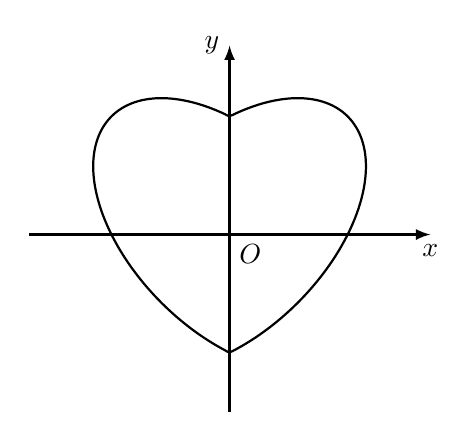
\begin{tikzpicture}[>=latex, scale=1.5]
  \draw[->, thick] (-1.7, 0) -- (1.7, 0) node[below] {$x$};
  \draw[->, thick] (0, -1.5) -- (0, 1.6) node[left] {$y$};
  \node[below right] at (0, 0) {$O$};

  \draw[thick, domain=0:360, samples=200, smooth]
    plot ({1/sqrt(1 - abs(cos(\x))*sin(\x)) * cos(\x)}, {1/sqrt(1 - abs(cos(\x))*sin(\x)) * sin(\x)});
\end{tikzpicture}
\end{center}
\nopagebreak[4]
(A) ①　(B) ②　(C) ①②　(D) ①②③

\Needspace{4\baselineskip}
\textbf{解析}

曲线方程为 $C: x^2 + y^2 = 1 + |x|y$。
因为将 $x$ 替换为 $-x$ 方程不变，所以曲线关于 $y$ 轴对称。
逐项分析三个结论：

\begin{itemize}
\item \textbf{结论 ①}：
\end{itemize}
  整点即 $x, y \in \mathbb{Z}$。
  将方程看作关于 $y$ 的一元二次方程：$y^2 - |x|y + (x^2 - 1) = 0$。
  判别式为 $\Delta = (|x|)^2 - 4(x^2 - 1) = 4 - 3x^2$。
  要使方程有实数解，必须 $\Delta \geqslant 0$，即 $4 - 3x^2 \geqslant 0 \implies x^2 \leqslant \dfrac{4}{3}$。
  因为 $x$ 为整数，所以只能取 $x = 0$ 或 $x = \pm 1$：
\begin{itemize}
\item 当 $x = 0$ 时，$y^2 = 1 \implies y = \pm 1$，得到整点 $(0, 1)$ 和 $(0, -1)$；
\item 当 $x = 1$ 时，$y^2 - y = 0 \implies y(y - 1) = 0 \implies y = 0$ 或 $y = 1$，得到整点 $(1, 0)$ 和 $(1, 1)$；
\item 当 $x = -1$ 时，由关于 $y$ 轴对称性，同理得到整点 $(-1, 0)$ 和 $(-1, 1)$。
\end{itemize}
  当 $|x| \geqslant 2$ 时，$\Delta < 0$，不存在任何实数解。
  因此曲线 $C$ 上的整点恰好只有上述 6 个，结论 ① 正确。

\begin{itemize}
\item \textbf{结论 ②}：
\end{itemize}
  设曲线上任意一点为 $(x, y)$，其到原点的距离为 $r = \sqrt{x^2 + y^2}$。
\Needspace{5\baselineskip}
  由基本不等式：
\nopagebreak[4]
\[|x|y \leqslant |x||y| \leqslant \frac{x^2 + y^2}{2} = \frac{r^2}{2}.\]
\Needspace{5\baselineskip}
  将曲线方程 $x^2 + y^2 = 1 + |x|y$ 代入，得：
\nopagebreak[4]
\[r^2 = 1 + |x|y \leqslant 1 + \frac{r^2}{2} \implies \frac{r^2}{2} \leqslant 1 \implies r^2 \leqslant 2 \implies r \leqslant \sqrt{2}.\]
  等号当且仅当 $|x| = y = 1$（即点 $(\pm 1, 1)$）时成立。
  因此曲线上任意一点到原点的距离都不超过 $\sqrt{2}$，结论 ② 正确。

\begin{itemize}
\item \textbf{结论 ③}：
\end{itemize}
\Needspace{5\baselineskip}
  由 $y^2 - |x|y + x^2 - 1 = 0$ 解得两支边界为：
\nopagebreak[4]
\[y = \frac{|x| \pm \sqrt{4 - 3x^2}}{2} \quad \left(|x| \leqslant \frac{2}{\sqrt{3}}\right).\]
\Needspace{5\baselineskip}
  曲线所围成的区域面积为垂直弦长的积分。由对称性：
\nopagebreak[4]
\[S = 2 \int_0^{\frac{2}{\sqrt{3}}} \left( \frac{x + \sqrt{4 - 3x^2}}{2} - \frac{x - \sqrt{4 - 3x^2}}{2} \right) \,\mathrm{d}x = 2 \int_0^{\frac{2}{\sqrt{3}}} \sqrt{4 - 3x^2} \,\mathrm{d}x.\]
\Needspace{5\baselineskip}
  提公因式 $\sqrt{3}$：
\nopagebreak[4]
\[S = 2\sqrt{3} \int_0^{\frac{2}{\sqrt{3}}} \sqrt{\left(\frac{2}{\sqrt{3}}\right)^2 - x^2} \,\mathrm{d}x.\]
\Needspace{5\baselineskip}
  利用圆面积的几何意义，定积分等于以 $\dfrac{2}{\sqrt{3}}$ 为半径的圆在第一象限的面积（即四分之一圆面积）：
\nopagebreak[4]
\[\int_0^{\frac{2}{\sqrt{3}}} \sqrt{\left(\frac{2}{\sqrt{3}}\right)^2 - x^2} \,\mathrm{d}x = \frac{1}{4} \pi \left(\frac{2}{\sqrt{3}}\right)^2 = \frac{\pi}{3}.\]
\Needspace{5\baselineskip}
  因此所求面积为：
\nopagebreak[4]
\[S = 2\sqrt{3} \times \frac{\pi}{3} = \frac{2\sqrt{3}\pi}{3} = \frac{2\pi}{\sqrt{3}} \approx \frac{2 \times 3.1416}{1.732} \approx 3.63 > 3.\]
  所以区域面积大于 3，结论 ③ 错误。

综上所述，所有正确结论的序号是 ①②。
故选 \textbf{C}。

\gkanswer{答案：C}

\par\medskip

\end{answer}
\gkpart{二、填空题}

\begin{answer}
\gksolhead{9}{}

\textbf{题目}：

函数 $f(x) = \sin^2 2x$ 的最小正周期是\gkblank{}.

\Needspace{4\baselineskip}
\textbf{解析}

\Needspace{5\baselineskip}
利用三角函数的降幂公式化简：
\nopagebreak[4]
\[f(x) = \sin^2 2x = \frac{1 - \cos 4x}{2} = -\frac{1}{2}\cos 4x + \frac{1}{2}.\]
由此可知函数 $f(x)$ 的角频率为 $\omega = 4$。
\Needspace{5\baselineskip}
所以最小正周期为：
\nopagebreak[4]
\[T = \frac{2\pi}{\omega} = \frac{2\pi}{4} = \frac{\pi}{2}.\]

\gkanswer{答案：$\dfrac{\pi}{2}$}

\end{answer}
\begin{answer}
\gksolhead{10}{}

\textbf{题目}：

设等差数列 $\{a_n\}$ 的前 $n$ 项和为 $S_n$, 若 $a_2 = -3$, $S_5 = -10$, 则 $a_5 =$\gkblank{}, $S_n$ 的最小值为\gkblank{}.

\Needspace{4\baselineskip}
\textbf{解析}

设等差数列 $\{a_n\}$ 的首项为 $a_1$，公差为 $d$。
\Needspace{5\baselineskip}
由前 $n$ 项和公式与性质，等差数列前 5 项和为：
\nopagebreak[4]
\[S_5 = \frac{5(a_1 + a_5)}{2} = 5a_3 = -10 \implies a_3 = -2.\]
\Needspace{5\baselineskip}
公差为：
\nopagebreak[4]
\[d = a_3 - a_2 = -2 - (-3) = 1.\]
\Needspace{5\baselineskip}
首项为：
\nopagebreak[4]
\[a_1 = a_2 - d = -3 - 1 = -4.\]
因此通项公式为 $a_n = a_1 + (n - 1)d = -4 + (n - 1) \times 1 = n - 5$。
\Needspace{5\baselineskip}
可得：
\nopagebreak[4]
\[a_5 = 5 - 5 = 0.\]
观察各项正负：$a_1 = -4 < 0$，$a_2 = -3 < 0$，$a_3 = -2 < 0$，$a_4 = -1 < 0$，$a_5 = 0$，$a_6 = 1 > 0$。
当 $n \leqslant 4$ 时，各项均为负数；第 5 项为 0；从第 6 项起各项均为正数。
\Needspace{5\baselineskip}
因此当 $n = 4$ 或 $n = 5$ 时，$S_n$ 取得最小值：
\nopagebreak[4]
\[S_4 = S_5 = -4 + (-3) + (-2) + (-1) + 0 = -10.\]

\gkanswer{答案：$0$；$-10$}

\end{answer}
\begin{answer}
\gksolhead{11}{}

\textbf{题目}：

某几何体是由一个正方体去掉一个四棱柱所得, 其三视图如图所示. 如果网格纸上小正方形的边长为 1, 那么该几何体的体积为\gkblank{}.
\nopagebreak[4]
\begin{center}\begin{tikzpicture}[>=latex, scale=0.45, font=\small]
  % 网格底图
  \draw[step=1, gray!50, very thin] (0, -1) grid (14, 10);

  % 正 (主) 视图
  \draw[thick] (2, 5) rectangle (6, 9);
  \draw[thick] (2, 6) -- (6, 6);
  \node[below] at (4, 4.8) {正 (主) 视图};

  % 侧 (左) 视图
  \draw[thick] (9, 5) -- (13, 5) -- (13, 6) -- (11, 6) -- (9, 9) -- cycle;
  \node[below] at (11, 4.8) {侧 (左) 视图};

  % 俯视图
  \draw[thick] (2, 0) rectangle (6, 4);
  \draw[thick] (2, 2) -- (6, 2);
  \node[below] at (4, -0.2) {俯视图};
\end{tikzpicture}
\end{center}
\nopagebreak[4]
\Needspace{4\baselineskip}
\textbf{解析}

由三视图可知：
原正方体的棱长为 4，体积为 $V_0 = 4^3 = 64$。
该几何体由正方体去掉一个四棱柱得到。
以侧（左）视图为截面，几何体是一个高（即主视图中的宽度）为 4 的柱体：
截面在 $4 \times 4$ 网格中的轮廓为五边形：
\begin{itemize}
\item 底边长为 4，左侧高为 4；
\item 右侧垂直边缘高为 1；
\item 顶部水平线段长为 2（从深度的 2 到 4，高度为 1）；
\item 倾斜线段连接点 $(0, 4)$ 与点 $(2, 1)$。
\end{itemize}
截面图形可分割为一个直角梯形和一个矩形：
\begin{itemize}
\item 梯形部分：上底为 1，下底为 4，高为 2，面积为 $\dfrac{1 + 4}{2} \times 2 = 5$；
\item 矩形部分：宽为 2，高为 1，面积为 $2 \times 1 = 2$。
\end{itemize}
截面总面积为 $S = 5 + 2 = 7$。
\Needspace{5\baselineskip}
因为柱体的高为 4，所以该几何体的体积为：
\nopagebreak[4]
\[V = S \times 4 = 7 \times 4 = 28.\]
（注：也可由去掉部分的体积计算：正方体上方切去的四棱柱截面为直角梯形，梯形上底为 2，下底为 4，高为 $4 - 1 = 3$，面积为 $\dfrac{2 + 4}{2} \times 3 = 9$。切去四棱柱体积为 $9 \times 4 = 36$。所求几何体体积为 $64 - 36 = 28$。）

\gkanswer{答案：$28$}

\end{answer}
\begin{answer}
\gksolhead{12}{}

\textbf{题目}：

已知 $l, m$ 是平面 $\alpha$ 外的两条不同直线. 给出下列三个论断:  
① $l \perp m$;  
② $m \parallel \alpha$;  
③ $l \perp \alpha$.  
以其中的两个论断作为条件, 余下的一个论断作为结论, 写出一个正确的命题: \gkblank{}.

\Needspace{4\baselineskip}
\textbf{解析}

考虑命题：若 $m \parallel \alpha$ 且 $l \perp \alpha$，则 $l \perp m$（即 ②③ $\implies$ ①）。
证明：
因为 $m \parallel \alpha$，所以在平面 $\alpha$ 内必存在一条直线 $m'$ 使得 $m' \parallel m$。
又因为 $l \perp \alpha$，且 $m' \subset \alpha$，所以 $l \perp m'$。
由 $m \parallel m'$ 且 $l \perp m'$，根据空间直线平行的传递性质，可得 $l \perp m$。
故 ②③ $\implies$ ① 成立。
（注：同理，若选 ①③ 为条件，由 $l \perp m$ 且 $l \perp \alpha$，因 $m$ 在平面 $\alpha$ 外，也可推出 $m \parallel \alpha$，即 ①③ $\implies$ ② 亦为正确命题。）

\gkanswer{答案：②③ $\implies$ ①（或 ①③ $\implies$ ②）}

\end{answer}
\begin{answer}
\gksolhead{13}{}

\textbf{题目}：

设函数 $f(x) = \mathrm{e}^x + a\mathrm{e}^{-x}$ ($a$ 为常数). 若 $f(x)$ 为奇函数, 则 $a =$\gkblank{}; 若 $f(x)$ 是 $\mathbb{R}$ 上的增函数, 则 $a$ 的取值范围是\gkblank{}.

\Needspace{4\baselineskip}
\textbf{解析}

函数为 $f(x) = \mathrm{e}^x + a\mathrm{e}^{-x}$。
\begin{itemize}
\item 若 $f(x)$ 为奇函数，其定义域为 $\mathbb{R}$，则必有 $f(0) = 0$：
\end{itemize}
\nopagebreak[4]
\[f(0) = \mathrm{e}^0 + a\mathrm{e}^0 = 1 + a = 0 \implies a = -1.\]
  检验：当 $a = -1$ 时，$f(x) = \mathrm{e}^x - \mathrm{e}^{-x}$，满足 $f(-x) = -f(x)$，确为奇函数。
\begin{itemize}
\item 若 $f(x)$ 是 $\mathbb{R}$ 上的增函数，求导得：
\end{itemize}
\nopagebreak[4]
\[f'(x) = \mathrm{e}^x - a\mathrm{e}^{-x}.\]
\Needspace{5\baselineskip}
  增函数要求导数在 $\mathbb{R}$ 上恒非负，即：
\nopagebreak[4]
\[\mathrm{e}^x - a\mathrm{e}^{-x} \geqslant 0 \iff a \leqslant \mathrm{e}^{2x} \quad (\forall x \in \mathbb{R}).\]
  因为对任意实数 $x$，都有 $\mathrm{e}^{2x} > 0$，且当 $x \to -\infty$ 时 $\mathrm{e}^{2x} \to 0$，
  所以要使 $a \leqslant \mathrm{e}^{2x}$ 恒成立，必须且只需 $a \leqslant 0$。
  此时 $f'(x) = \mathrm{e}^x - a\mathrm{e}^{-x} > 0$（当 $a < 0$ 时）或 $f'(x) = \mathrm{e}^x > 0$（当 $a = 0$ 时），函数严格单调递增。
  故 $a$ 的取值范围是 $(-\infty, 0]$（或 $a \leqslant 0$）。

\gkanswer{答案：$-1$；$(-\infty, 0]$（或 $a \leqslant 0$）}

\end{answer}
\begin{answer}
\gksolhead{14}{}

\textbf{题目}：

李明自主创业, 在网上经营一家水果店, 销售的水果中有草莓、京白梨、西瓜、桃, 价格依次为 60 元/盒、65 元/盒、80 元/盒、90 元/盒. 为增加销量, 李明对这四种水果进行促销: 一次购买水果的总价达到 120 元, 顾客就少付 $x$ 元. 每笔订单顾客网上支付成功后, 李明会得到支付款的 80\\%.  
① 当 $x = 10$ 时, 顾客一次购买草莓和西瓜各 1 盒, 需要支付\gkblank{}元;  
② 在促销活动中, 为保证李明每笔订单得到的金额均不低于促销前总价的七折, 则 $x$ 的最大值为\gkblank{}.

\Needspace{4\baselineskip}
\textbf{解析}

促销规则：一次购买水果总价达到 120 元少付 $x$ 元；李明获得支付款的 80\\%。
\begin{itemize}
\item \textbf{① 的解析}：
\end{itemize}
  草莓 60 元/盒，西瓜 80 元/盒。
  购买草莓和西瓜各 1 盒的原总价为 $60 + 80 = 140$ 元。
  因为 $140 \geqslant 120$，达到促销标准，当 $x = 10$ 时，顾客少付 10 元。
\Needspace{5\baselineskip}
  顾客实际需要支付：
\nopagebreak[4]
\[140 - 10 = 130\text{ \text{元}}.\]
\begin{itemize}
\item \textbf{② 的解析}：
\end{itemize}
  设订单原总价为 $P$。
  当 $P \geqslant 120$ 时，顾客支付金额为 $P - x$ 元。
  李明实际获得的金额为 $0.8(P - x)$ 元。
\Needspace{5\baselineskip}
  要求每笔订单得到的金额均不低于原总价的七折（即 $0.7P$），则：
\nopagebreak[4]
\[0.8(P - x) \geqslant 0.7P \iff 0.8P - 0.8x \geqslant 0.7P \iff 0.1P \geqslant 0.8x \iff x \leqslant \frac{P}{8}.\]
  要保证该条件对所有达到促销门槛的订单都成立，必须 $x \leqslant \dfrac{P_{\min}}{8}$。
  水果单价为 60、65、80、90 元/盒。
  达到促销门槛 120 元的最小总价为购买 2 盒草莓：$60 \times 2 = 120$ 元，即 $P_{\min} = 120$ 元。
\Needspace{5\baselineskip}
  因此：
\nopagebreak[4]
\[x \leqslant \frac{120}{8} = 15.\]
  所以 $x$ 的最大值为 15。

\gkanswer{答案：① $130$；② $15$}

\par\medskip

\end{answer}
\gkpart{三、解答题}

\begin{answer}
\gksolhead{15}{}

\textbf{题目}（13 分）：

在 $\triangle ABC$ 中, $a = 3$, $b - c = 2$, $\cos B = -\dfrac{1}{2}$.

(1) 求 $b, c$ 的值;  
(2) 求 $\sin (B - C)$ 的值.

\Needspace{4\baselineskip}
\textbf{解析}

在 $\triangle ABC$ 中，$a = 3, b - c = 2, \cos B = -\dfrac{1}{2}$。

\textbf{(1) 解析}
\Needspace{5\baselineskip}
由余弦定理 $b^2 = a^2 + c^2 - 2ac\cos B$，代入 $a = 3, \cos B = -\dfrac{1}{2}$ 得：
\nopagebreak[4]
\[b^2 = 3^2 + c^2 - 2 \times 3 \times c \times \left(-\frac{1}{2}\right) = 9 + c^2 + 3c.\]
由已知 $b - c = 2$ 可得 $b = c + 2$。
\Needspace{5\baselineskip}
将 $b = c + 2$ 代入上式，得：
\nopagebreak[4]
\[(c + 2)^2 = c^2 + 3c + 9.\]
\Needspace{5\baselineskip}
展开化简：
\nopagebreak[4]
\[c^2 + 4c + 4 = c^2 + 3c + 9 \implies c = 5.\]
\Needspace{5\baselineskip}
从而：
\nopagebreak[4]
\[b = c + 2 = 7.\]
故 $b = 7, c = 5$。

\textbf{(2) 解析}
因为 $\cos B = -\dfrac{1}{2}$，且 $0 < B < \pi$，
所以 $B = \dfrac{2\pi}{3}$，$\sin B = \dfrac{\sqrt{3}}{2}$。
\Needspace{5\baselineskip}
在 $\triangle ABC$ 中由正弦定理 $\dfrac{b}{\sin B} = \dfrac{c}{\sin C}$，得：
\nopagebreak[4]
\[\sin C = \frac{c\sin B}{b} = \frac{5 \times \frac{\sqrt{3}}{2}}{7} = \frac{5\sqrt{3}}{14}.\]
因为 $B = \dfrac{2\pi}{3} > \dfrac{\pi}{2}$，所以角 $C$ 必为锐角，从而 $\cos C > 0$。
\Needspace{5\baselineskip}
因此：
\nopagebreak[4]
\[\cos C = \sqrt{1 - \sin^2 C} = \sqrt{1 - \left(\frac{5\sqrt{3}}{14}\right)^2} = \sqrt{1 - \frac{75}{196}} = \sqrt{\frac{121}{196}} = \frac{11}{14}.\]
\Needspace{5\baselineskip}
由两角差的正弦公式：
\nopagebreak[4]
\[\sin(B - C) = \sin B\cos C - \cos B\sin C.\]
\Needspace{5\baselineskip}
代入各三角函数值：
\nopagebreak[4]
\[\sin(B - C) = \frac{\sqrt{3}}{2} \times \frac{11}{14} - \left(-\frac{1}{2}\right) \times \frac{5\sqrt{3}}{14} = \frac{11\sqrt{3}}{28} + \frac{5\sqrt{3}}{28} = \frac{16\sqrt{3}}{28} = \frac{4\sqrt{3}}{7}.\]

\gkanswer{答案（1）：$b = 7, c = 5$}

\gkanswer{答案（2）：$\dfrac{4\sqrt{3}}{7}$}

\end{answer}
\begin{answer}
\gksolhead{16}{}

\textbf{题目}（14 分）：

如图, 在四棱锥 $P - ABCD$ 中, $PA \perp$ 平面 $ABCD$, $AD \perp CD$, $AD \parallel BC$, $PA = AD = CD = 2$, $BC = 3$. $E$ 为 $PD$ 的中点, 点 $F$ 在 $PC$ 上, 且 $\dfrac{PF}{PC} = \dfrac{1}{3}$.
\nopagebreak[4]
\begin{center}\begin{tikzpicture}[>=latex, scale=1.1, font=\small]
  \coordinate (A) at (0, 0);
  \coordinate (D) at (3.0, 0);
  \coordinate (B) at (-2.4, -1.0);
  \coordinate (C) at (1.8, -1.0);
  \coordinate (P) at (0, 3.0);

  % 点 E 为 PD 中点
  \coordinate (E) at ($(P)!0.5!(D)$);
  % 点 F 在 PC 上，PF/PC = 1/3
  \coordinate (F) at ($(P)!0.333!(C)$);
  % 点 G 在 PB 上，PG/PB = 2/3
  \coordinate (G) at ($(P)!0.667!(B)$);

  % 虚线边（内部不可见线段）
  \draw[dashed, thin] (P) -- (A);
  \draw[dashed, thin] (A) -- (B);
  \draw[dashed, thin] (A) -- (D);
  \draw[dashed, thin] (A) -- (E);
  \draw[dashed, thin] (A) -- (F);
  \draw[dashed, thin] (A) -- (G);

  % 实线边（外轮廓与可见边）
  \draw[thick] (P) -- (B) -- (C) -- (D) -- (P);
  \draw[thick] (P) -- (C);
  \draw[thick] (E) -- (F);

  % 顶点标签
  \node[above] at (P) {$P$};
  \node[below] at (A) {$A$};
  \node[below left] at (B) {$B$};
  \node[below right] at (C) {$C$};
  \node[right] at (D) {$D$};
  \node[above right] at (E) {$E$};
  \node[left] at (F) {$F$};
  \node[left] at (G) {$G$};
\end{tikzpicture}
\end{center}
\nopagebreak[4]
(1) 求证: $CD \perp$ 平面 $PAD$;  
(2) 求二面角 $F - AE - P$ 的余弦值;  
(3) 设点 $G$ 在 $PB$ 上, 且 $\dfrac{PG}{PB} = \dfrac{2}{3}$. 判断直线 $AG$ 是否在平面 $AEF$ 内, 说明理由.

\Needspace{4\baselineskip}
\textbf{解析}

四棱锥 $P - ABCD$ 中，$PA \perp$ 平面 $ABCD$，$AD \perp CD$，$AD \parallel BC$，$PA = AD = CD = 2$，$BC = 3$。

\textbf{(1) 解析}
因为 $PA \perp$ 平面 $ABCD$，且 $CD \subset$ 平面 $ABCD$，
所以 $PA \perp CD$。
又已知 $AD \perp CD$，即 $CD \perp AD$。
因为 $PA \subset$ 平面 $PAD$，$AD \subset$ 平面 $PAD$，且 $PA \cap AD = A$，
所以 $CD \perp$ 平面 $PAD$。

\textbf{(2) 解析}
由 (1) 知，$PA, AD, CD$ 两两垂直。
以点 $A$ 为坐标原点建立空间直角坐标系：
\begin{itemize}
\item 射线 $AD$ 为 $x$ 轴正方向；
\item 在底面内过点 $A$ 作平行于 $CD$ 的射线为 $y$ 轴正方向；
\item 射线 $AP$ 为 $z$ 轴正方向。
\end{itemize}
\Needspace{5\baselineskip}
由已知长度可得各点坐标：
\nopagebreak[4]
\[A(0, 0, 0), \quad D(2, 0, 0), \quad P(0, 0, 2).\]
因为 $CD \parallel y$ 轴且 $CD = 2$，所以 $C(2, 2, 0)$。
因为 $AD \parallel BC$ 且 $BC = 3$，向量 $\vec{CB}$ 与 $\vec{DA} = (-2, 0, 0)$ 同向，所以 $B(-1, 2, 0)$。
\Needspace{5\baselineskip}
点 $E$ 为线段 $PD$ 的中点，由中点坐标公式：
\nopagebreak[4]
\[E(1, 0, 1).\]
\Needspace{5\baselineskip}
点 $F$ 在 $PC$ 上，且 $\dfrac{PF}{PC} = \dfrac{1}{3}$：
\nopagebreak[4]
\[\vec{PF} = \frac{1}{3}\vec{PC} = \frac{1}{3}(2, 2, -2) = \left(\frac{2}{3}, \frac{2}{3}, -\frac{2}{3}\right),\]
\Needspace{5\baselineskip}
故点 $F$ 坐标为：
\nopagebreak[4]
\[F = P + \vec{PF} = \left(\frac{2}{3}, \frac{2}{3}, \frac{4}{3}\right).\]
\Needspace{5\baselineskip}
平面 $PAD$ 即为 $xz$ 平面，其一个法向量为：
\nopagebreak[4]
\[\boldsymbol{n}_1 = (0, 1, 0).\]
设平面 $AEF$ 的法向量为 $\boldsymbol{n}_2 = (x, y, z)$。
\Needspace{5\baselineskip}
由 $\vec{AE} = (1, 0, 1)$，$\vec{AF} = \left(\dfrac{2}{3}, \dfrac{2}{3}, \dfrac{4}{3}\right)$：
\nopagebreak[4]
\[\begin{cases} \boldsymbol{n}_2 \cdot \vec{AE} = x + z = 0, \\ \boldsymbol{n}_2 \cdot \vec{AF} = \dfrac{2}{3}x + \dfrac{2}{3}y + \dfrac{4}{3}z = 0 \implies x + y + 2z = 0. \end{cases}\]
取 $z = -1$，则 $x = 1$。代入第二式得 $1 + y - 2 = 0 \implies y = 1$。
故平面 $AEF$ 的一个法向量为 $\boldsymbol{n}_2 = (1, 1, -1)$。
\Needspace{5\baselineskip}
计算两法向量夹角的余弦值：
\nopagebreak[4]
\[\cos\langle\boldsymbol{n}_1, \boldsymbol{n}_2\rangle = \frac{\boldsymbol{n}_1 \cdot \boldsymbol{n}_2}{|\boldsymbol{n}_1||\boldsymbol{n}_2|} = \frac{0 \times 1 + 1 \times 1 + 0 \times (-1)}{1 \times \sqrt{1^2 + 1^2 + (-1)^2}} = \frac{1}{\sqrt{3}} = \frac{\sqrt{3}}{3}.\]
由图形可知二面角 $F - AE - P$ 为锐角，
所以二面角 $F - AE - P$ 的余弦值为 $\dfrac{\sqrt{3}}{3}$。

\textbf{(3) 解析}
直线 $AG$ 在平面 $AEF$ 内。理由如下：
由已知，点 $G$ 在 $PB$ 上，且 $\dfrac{PG}{PB} = \dfrac{2}{3}$。
\Needspace{5\baselineskip}
因为 $P(0, 0, 2)$，$B(-1, 2, 0)$，所以：
\nopagebreak[4]
\[\vec{PG} = \frac{2}{3}\vec{PB} = \frac{2}{3}(-1, 2, -2) = \left(-\frac{2}{3}, \frac{4}{3}, -\frac{4}{3}\right).\]
\Needspace{5\baselineskip}
从而点 $G$ 的坐标为：
\nopagebreak[4]
\[G = P + \vec{PG} = \left(-\frac{2}{3}, \frac{4}{3}, \frac{2}{3}\right).\]
向量 $\vec{AG} = \left(-\dfrac{2}{3}, \dfrac{4}{3}, \dfrac{2}{3}\right)$。
\Needspace{5\baselineskip}
计算 $\vec{AG}$ 与平面 $AEF$ 的法向量 $\boldsymbol{n}_2 = (1, 1, -1)$ 的数量积：
\nopagebreak[4]
\[\boldsymbol{n}_2 \cdot \vec{AG} = 1 \times \left(-\frac{2}{3}\right) + 1 \times \frac{4}{3} + (-1) \times \frac{2}{3} = -\frac{2}{3} + \frac{4}{3} - \frac{2}{3} = 0.\]
这说明向量 $\vec{AG} \perp \boldsymbol{n}_2$。
又因为直线 $AG$ 经过平面 $AEF$ 内的点 $A$，
所以直线 $AG$ 在平面 $AEF$ 内。

\gkanswer{答案（1）：证明见解析}

\gkanswer{答案（2）：$\dfrac{\sqrt{3}}{3}$}

\gkanswer{答案（3）：直线 $AG$ 在平面 $AEF$ 内，理由见解析}

\end{answer}
\begin{answer}
\gksolhead{17}{}

\textbf{题目}（13 分）：

改革开放以来, 人们的支付方式发生了巨大转变. 近年来, 移动支付已成为主要支付方式之一. 为了解某校学生上个月 A, B 两种移动支付方式的使用情况, 从全校学生中随机抽取了 100 人, 发现样本中 A, B 两种支付方式都不使用的有 5 人, 样本中仅使用 A 和仅使用 B 的学生的支付金额分布情况如下:

\begin{center}
\begin{tabular}{llll}
\toprule
支付金额 (元) \ 支付方式 & $(0, 1000]$ & $(1000, 2000]$ & 大于 2000 \\
\midrule
仅使用 A & 18 人 & 9 人 & 3 人 \\
仅使用 B & 10 人 & 14 人 & 1 人 \\
\bottomrule
\end{tabular}
\end{center}

(1) 从全校学生中随机抽取 1 人, 估计该学生上个月 A, B 两种支付方式都使用的概率;  
(2) 从样本仅使用 A 和仅使用 B 的学生中各随机抽取 1 人, 以 $X$ 表示这 2 人中上个月支付金额大于 1000 元的人数, 求 $X$ 的分布列和数学期望;  
(3) 已知上个月样本学生的支付方式在本月没有变化. 现从样本仅使用 A 的学生中, 随机抽查 3 人, 发现他们本月的支付金额都大于 2000 元. 根据抽查结果, 能否认为样本仅使用 A 的学生中本月支付金额大于 2000 元的人数有变化? 说明理由.

\Needspace{4\baselineskip}
\textbf{解析}

调查样本容量为 100 人，两种支付方式都不使用的有 5 人。
仅使用 A 的学生总人数为 $18 + 9 + 3 = 30$ 人。
仅使用 B 的学生总人数为 $10 + 14 + 1 = 25$ 人。

\textbf{(1) 解析}
\Needspace{5\baselineskip}
在 100 人的样本中，A, B 两种支付方式都使用的学生人数为：
\nopagebreak[4]
\[100 - 5 - 30 - 25 = 40\text{ \text{人}}.\]
\Needspace{5\baselineskip}
因此，从全校学生中随机抽取 1 人，估计该学生上个月 A, B 两种支付方式都使用的概率为：
\nopagebreak[4]
\[P = \frac{40}{100} = 0.4.\]

\textbf{(2) 解析}
在样本仅使用 A 的 30 人中，支付金额大于 1000 元的人数为 $9 + 3 = 12$ 人。
从中随机抽取 1 人，支付金额大于 1000 元的概率为 $p_1 = \dfrac{12}{30} = \dfrac{2}{5}$。
在样本仅使用 B 的 25 人中，支付金额大于 1000 元的人数为 $14 + 1 = 15$ 人。
从中随机抽取 1 人，支付金额大于 1000 元的概率为 $p_2 = \dfrac{15}{25} = \dfrac{3}{5}$。
由题意，随机变量 $X$ 的可能取值为 $0, 1, 2$。
\Needspace{5\baselineskip}
计算各取值的概率：
\nopagebreak[4]
\[P(X = 0) = (1 - p_1)(1 - p_2) = \left(1 - \frac{2}{5}\right)\left(1 - \frac{3}{5}\right) = \frac{3}{5} \times \frac{2}{5} = \frac{6}{25},\]
\nopagebreak[4]
\[P(X = 1) = p_1(1 - p_2) + (1 - p_1)p_2 = \frac{2}{5} \times \frac{2}{5} + \frac{3}{5} \times \frac{3}{5} = \frac{4}{25} + \frac{9}{25} = \frac{13}{25},\]
\nopagebreak[4]
\[P(X = 2) = p_1 p_2 = \frac{2}{5} \times \frac{3}{5} = \frac{6}{25}.\]
所以 $X$ 的分布列为：

\begin{center}
\begin{tabular}{llll}
\toprule
$X$ & 0 & 1 & 2 \\
\midrule
$P$ & $\dfrac{6}{25}$ & $\dfrac{13}{25}$ & $\dfrac{6}{25}$ \\
\bottomrule
\end{tabular}
\end{center}

\Needspace{5\baselineskip}
$X$ 的数学期望为：
\nopagebreak[4]
\[E(X) = 0 \times \frac{6}{25} + 1 \times \frac{13}{25} + 2 \times \frac{6}{25} = \frac{25}{25} = 1.\]

\textbf{(3) 解析}
能够认为样本仅使用 A 的学生中本月支付金额大于 2000 元的人数有变化。理由如下：
上个月样本仅使用 A 的 30 人中，支付金额大于 2000 元的仅有 3 人。
假设本月支付金额大于 2000 元的人数没有变化（仍为 3 人），
\Needspace{5\baselineskip}
现从这 30 人中随机抽查 3 人，这 3 人的支付金额都大于 2000 元的概率为：
\nopagebreak[4]
\[P = \frac{\binom{3}{3}}{\binom{30}{3}} = \frac{1}{\frac{30 \times 29 \times 28}{3 \times 2 \times 1}} = \frac{1}{4060} \approx 0.00025.\]
根据假设检验小概率事件原理，概率极小的事件在一次试验中几乎不可能发生。
而在本次实际抽查中该事件确实发生了，因此有充分理由认为原假设不成立，即样本仅使用 A 的学生中本月支付金额大于 2000 元的人数发生了变化（增加）。

\gkanswer{答案（1）：$0.4$}

\gkanswer{答案（2）：分布列见解析，$E(X) = 1$}

\gkanswer{答案（3）：能认为有变化，理由见解析}

\end{answer}
\begin{answer}
\gksolhead{18}{}

\textbf{题目}（14 分）：

已知抛物线 $C: x^2 = -2py$ 经过点 $(2, -1)$.

(1) 求抛物线 $C$ 的方程及其准线方程;  
(2) 设 $O$ 为原点, 过抛物线 $C$ 的焦点作斜率不为 0 的直线 $l$ 交抛物线 $C$ 于两点 $M, N$, 直线 $y = -1$ 分别交直线 $OM, ON$ 于点 $A$ 和点 $B$. 求证: 以 $AB$ 为直径的圆经过 $y$ 轴上的两个定点.

\Needspace{4\baselineskip}
\textbf{解析}

抛物线 $C: x^2 = -2py$ ($p > 0$) 经过点 $(2, -1)$。

\textbf{(1) 解析}
\Needspace{5\baselineskip}
将点 $(2, -1)$ 代入抛物线方程：
\nopagebreak[4]
\[2^2 = -2p \times (-1) \implies 4 = 2p \implies p = 2.\]
所以抛物线 $C$ 的方程为 $x^2 = -4y$。
其准线方程为 $y = \dfrac{p}{2} = 1$。

\textbf{(2) 解析}
由 (1) 知抛物线焦点为 $F(0, -1)$。
设过焦点 $F(0, -1)$ 且斜率不为 0 的直线 $l$ 的方程为 $y = kx - 1$ ($k \neq 0$)。
\Needspace{5\baselineskip}
联立直线 $l$ 与抛物线方程：
\nopagebreak[4]
\[\begin{cases} y = kx - 1, \\ x^2 = -4y, \end{cases} \implies x^2 = -4(kx - 1) \implies x^2 + 4kx - 4 = 0.\]
判别式 $\Delta = (4k)^2 - 4(-4) = 16k^2 + 16 > 0$ 恒成立。
\Needspace{5\baselineskip}
设交点坐标为 $M(x_1, y_1)$，$N(x_2, y_2)$，由韦达定理：
\nopagebreak[4]
\[x_1 + x_2 = -4k, \quad x_1 x_2 = -4.\]
直线 $OM$ 的斜率为 $\dfrac{y_1}{x_1} = -\dfrac{x_1}{4}$，直线方程为 $y = -\dfrac{x_1}{4}x$。
\Needspace{5\baselineskip}
令 $y = -1$，解得点 $A$ 的横坐标：
\nopagebreak[4]
\[-1 = -\frac{x_1}{4}x_A \implies x_A = \frac{4}{x_1}.\]
故点 $A$ 的坐标为 $\left(\dfrac{4}{x_1}, -1\right)$。
同理，直线 $ON$ 的方程为 $y = -\dfrac{x_2}{4}x$，令 $y = -1$ 得点 $B$ 的坐标为 $\left(\dfrac{4}{x_2}, -1\right)$。
\Needspace{5\baselineskip}
线段 $AB$ 的两端点均在直线 $y = -1$ 上，以 $AB$ 为直径的圆的方程为：
\nopagebreak[4]
\[\left(x - \frac{x_A + x_B}{2}\right)^2 + (y + 1)^2 = \left(\frac{x_A - x_B}{2}\right)^2.\]
\Needspace{5\baselineskip}
展开整理得：
\nopagebreak[4]
\[x^2 - (x_A + x_B)x + x_A x_B + (y + 1)^2 = 0.\]
\Needspace{5\baselineskip}
计算系数：
\nopagebreak[4]
\[x_A x_B = \frac{4}{x_1} \cdot \frac{4}{x_2} = \frac{16}{x_1 x_2} = \frac{16}{-4} = -4,\]
\nopagebreak[4]
\[x_A + x_B = \frac{4}{x_1} + \frac{4}{x_2} = \frac{4(x_1 + x_2)}{x_1 x_2} = \frac{4(-4k)}{-4} = 4k.\]
\Needspace{5\baselineskip}
代入圆的方程得：
\nopagebreak[4]
\[x^2 - 4kx - 4 + (y + 1)^2 = 0.\]
\Needspace{5\baselineskip}
令 $x = 0$，得：
\nopagebreak[4]
\[(y + 1)^2 - 4 = 0 \implies (y + 1)^2 = 4 \implies y + 1 = \pm 2.\]
解得 $y = 1$ 或 $y = -3$。
该式与参数 $k$ 无关，表明无论直线 $l$ 的斜率 $k$ 为何非零实数，以 $AB$ 为直径的圆恒经过 $y$ 轴上的两个定点 $(0, 1)$ 和 $(0, -3)$。

\gkanswer{答案（1）：抛物线 $C$ 的方程为 $x^2 = -4y$，准线方程为 $y = 1$}

\gkanswer{答案（2）：证明见解析，定点坐标为 $(0, 1)$ 和 $(0, -3)$}

\end{answer}
\begin{answer}
\gksolhead{19}{}

\textbf{题目}（13 分）：

已知函数 $f(x) = \dfrac{1}{4}x^3 - x^2 + x$.

(1) 求曲线 $y = f(x)$ 的斜率为 1 的切线方程;  
(2) 当 $x \in [-2, 4]$ 时, 求证: $x - 6 \leqslant f(x) \leqslant x$;  
(3) 设 $F(x) = |f(x) - (x + a)|$ ($a \in \mathbb{R}$), 记 $F(x)$ 在区间 $[-2, 4]$ 上的最大值为 $M(a)$. 当 $M(a)$ 最小时, 求 $a$ 的值.

\Needspace{4\baselineskip}
\textbf{解析}

已知函数 $f(x) = \dfrac{1}{4}x^3 - x^2 + x$。

\textbf{(1) 解析}
\Needspace{5\baselineskip}
对 $f(x)$ 求导得：
\nopagebreak[4]
\[f'(x) = \frac{3}{4}x^2 - 2x + 1.\]
\Needspace{5\baselineskip}
令切线斜率 $f'(x) = 1$，得：
\nopagebreak[4]
\[\frac{3}{4}x^2 - 2x + 1 = 1 \implies \frac{3}{4}x^2 - 2x = 0 \implies x\left(\frac{3}{4}x - 2\right) = 0.\]
解得切点横坐标为 $x = 0$ 或 $x = \dfrac{8}{3}$。
\begin{itemize}
\item 当 $x = 0$ 时，$f(0) = 0$，切点为 $(0, 0)$，切线方程为 $y - 0 = 1(x - 0) \implies y = x$；
\item 当 $x = \dfrac{8}{3}$ 时：
\end{itemize}
\nopagebreak[4]
\[f\left(\frac{8}{3}\right) = \frac{1}{4}\left(\frac{8}{3}\right)^3 - \left(\frac{8}{3}\right)^2 + \frac{8}{3} = \frac{128}{27} - \frac{64}{9} + \frac{8}{3} = \frac{8}{27}.\]
\Needspace{5\baselineskip}
  切点为 $\left(\dfrac{8}{3}, \dfrac{8}{27}\right)$，切线方程为：
\nopagebreak[4]
\[y - \frac{8}{27} = 1 \times \left(x - \frac{8}{3}\right) \implies y = x - \frac{64}{27}.\]
综上，曲线 $y = f(x)$ 的斜率为 1 的切线方程为 $y = x$ 或 $y = x - \dfrac{64}{27}$。

\textbf{(2) 解析}
证明：设 $h(x) = f(x) - x = \dfrac{1}{4}x^3 - x^2$。
\Needspace{5\baselineskip}
要证当 $x \in [-2, 4]$ 时 $x - 6 \leqslant f(x) \leqslant x$，等价于证明：
\nopagebreak[4]
\[-6 \leqslant h(x) \leqslant 0 \quad (\forall x \in [-2, 4]).\]
\Needspace{5\baselineskip}
对 $h(x)$ 求导：
\nopagebreak[4]
\[h'(x) = \frac{3}{4}x^2 - 2x = \frac{1}{4}x(3x - 8).\]
令 $h'(x) = 0$，解得在区间 $[-2, 4]$ 内的驻点为 $x = 0$ 和 $x = \dfrac{8}{3}$。
列表分析 $h(x)$ 在 $[-2, 4]$ 上的单调性：
\begin{itemize}
\item 当 $x \in [-2, 0)$ 时，$h'(x) > 0$，$h(x)$ 单调递增；
\item 当 $x \in \left(0, \dfrac{8}{3}\right)$ 时，$h'(x) < 0$，$h(x)$ 单调递减；
\item 当 $x \in \left(\dfrac{8}{3}, 4\right]$ 时，$h'(x) > 0$，$h(x)$ 单调递增。
\end{itemize}
\Needspace{5\baselineskip}
计算区间端点与极值点的函数值：
\nopagebreak[4]
\[h(-2) = \frac{1}{4}(-2)^3 - (-2)^2 = -2 - 4 = -6,\]
\nopagebreak[4]
\[h(0) = 0,\]
\nopagebreak[4]
\[h\left(\frac{8}{3}\right) = \frac{1}{4}\left(\frac{8}{3}\right)^2 \left(\frac{8}{3} - 4\right) = \frac{16}{9} \times \left(-\frac{4}{3}\right) = -\frac{64}{27},\]
\nopagebreak[4]
\[h(4) = \frac{1}{4}(4)^3 - 4^2 = 16 - 16 = 0.\]
由此可知，$h(x)$ 在 $[-2, 4]$ 上的最大值为 $h(0) = h(4) = 0$；
最小值为 $h(-2) = -6$（因为 $-6 < -\dfrac{64}{27}$）。
因此，对任意 $x \in [-2, 4]$ 均有 $-6 \leqslant h(x) \leqslant 0$。
即 $x - 6 \leqslant f(x) \leqslant x$ 成立。

\textbf{(3) 解析}
由 (2) 知，当 $x \in [-2, 4]$ 时，$f(x) - x = h(x)$ 的值域为 $[-6, 0]$。
函数 $F(x) = |f(x) - (x + a)| = |h(x) - a|$。
\Needspace{5\baselineskip}
因此 $F(x)$ 在区间 $[-2, 4]$ 上的最大值为：
\nopagebreak[4]
\[M(a) = \max_{x \in [-2, 4]} |h(x) - a| = \max\{|h_{\max} - a|, |h_{\min} - a|\} = \max\{|0 - a|, |-6 - a|\} = \max\{|a|, |a + 6|\}.\]
\Needspace{5\baselineskip}
由绝对值三角不等式：
\nopagebreak[4]
\[\max\{|a|, |a + 6|\} \geqslant \frac{|a| + |a + 6|}{2} \geqslant \frac{|-a + (a + 6)|}{2} = \frac{6}{2} = 3.\]
\Needspace{5\baselineskip}
等号当且仅当 $|a| = |a + 6|$ 且 $-a(a + 6) \geqslant 0$ 时成立，解得：
\nopagebreak[4]
\[-a = a + 6 \implies 2a = -6 \implies a = -3.\]
此时 $M(-3) = \max\{|-3|, |3|\} = 3$ 取得最小值。
所以当 $M(a)$ 最小时，$a = -3$。

\gkanswer{答案（1）：$y = x$ 或 $y = x - \dfrac{64}{27}$}

\gkanswer{答案（2）：证明见解析}

\gkanswer{答案（3）：$a = -3$}

\end{answer}
\begin{answer}
\gksolhead{20}{}

\textbf{题目}（13 分）：

已知数列 $\{a_n\}$ 从中选取第 $i_1$ 项、第 $i_2$ 项、$\cdots$、第 $i_m$ 项 ($i_1 < i_2 < \cdots < i_m$), 若 $a_{i_1} < a_{i_2} < \cdots < a_{i_m}$, 则称新数列 $a_{i_1}, a_{i_2}, \cdots, a_{i_m}$ 为 $\{a_n\}$ 的长度为 $m$ 的递增子列. 规定: 数列 $\{a_n\}$ 的任意一项都是 $\{a_n\}$ 的长度为 1 的递增子列.

(1) 写出数列 $1, 8, 3, 7, 5, 6, 9$ 的一个长度为 4 的递增子列;  
(2) 已知数列 $\{a_n\}$ 的长度为 $p$ 的递增子列的末项的最小值为 $a_{m_0}$, 长度为 $q$ 的递增子列的末项的最小值为 $a_{n_0}$. 若 $p < q$, 求证: $a_{m_0} < a_{n_0}$;  
(3) 设无穷数列 $\{a_n\}$ 的各项均为正整数, 且任意两项均不相等. 若 $\{a_n\}$ 的长度为 $s$ 的递增子列末项的最小值为 $2s - 1$, 且长度为 $s$ 末项为 $2s - 1$ 的递增子列恰有 $2^{s-1}$ 个 ($s = 1, 2, \cdots$), 求数列 $\{a_n\}$ 的通项公式.

\Needspace{4\baselineskip}
\textbf{解析}

递增子列定义：$a_{i_1} < a_{i_2} < \dots < a_{i_m}$ ($i_1 < i_2 < \dots < i_m$)。

\textbf{(1) 解析}
数列为 $1, 8, 3, 7, 5, 6, 9$。
选取其中递增的 4 项，例如：$1, 3, 5, 6$（对应项数为第 1, 3, 5, 6 项）。
（注：也可写出 $1, 3, 5, 9$ 或 $1, 3, 7, 9$ 或 $1, 5, 6, 9$ 或 $3, 5, 6, 9$ 等任一符合要求的长度为 4 的递增子列）。

\textbf{(2) 解析}
证明：
\Needspace{5\baselineskip}
由题意，数列 $\{a_n\}$ 存在长度为 $q$ 的递增子列，设其末项为最小值 $a_{n_0}$ 的一个递增子列为：
\nopagebreak[4]
\[a_{j_1} < a_{j_2} < \dots < a_{j_p} < \dots < a_{j_q} = a_{n_0} \quad (j_1 < j_2 < \dots < j_p < \dots < j_q).\]
\Needspace{5\baselineskip}
因为 $p < q$，在前 $q$ 项中截取前 $p$ 项：
\nopagebreak[4]
\[a_{j_1} < a_{j_2} < \dots < a_{j_p}.\]
根据定义，这构成了一个长度为 $p$ 的递增子列，其末项为 $a_{j_p}$。
\Needspace{5\baselineskip}
又已知长度为 $p$ 的递增子列末项的最小值为 $a_{m_0}$，故必有：
\nopagebreak[4]
\[a_{m_0} \leqslant a_{j_p}.\]
\Needspace{5\baselineskip}
而在该长度为 $q$ 的递增子列中，由于各项严格单调递增，且 $p < q$，所以：
\nopagebreak[4]
\[a_{j_p} < a_{j_q} = a_{n_0}.\]
\Needspace{5\baselineskip}
因此：
\nopagebreak[4]
\[a_{m_0} \leqslant a_{j_p} < a_{n_0} \implies a_{m_0} < a_{n_0}.\]
命题得证。

\textbf{(3) 解析}
数列 $\{a_n\}$ 的各项均为正整数且两两不相等。
\begin{itemize}
\item 当 $s = 1$ 时，长度为 1 的递增子列末项最小值为 $2(1) - 1 = 1$，且恰有 $2^0 = 1$ 个。
\end{itemize}
  因为数列中任意一项都是长度为 1 的递增子列，这表明数 1 是数列中所有项的最小值，且在数列中恰好出现 1 次。
\begin{itemize}
\item 由 (2) 的结论，长度为 $s$ 的递增子列末项最小值随着长度 $s$ 严格单调递增。
\end{itemize}
  对于任意正整数 $s$，长度为 $s$ 的递增子列末项最小值为 $2s - 1$。
  特别地，集合 $\{1, 3, 5, \dots, 2s - 1\}$ 中的所有数都是递增子列末项的最小值。
\begin{itemize}
\item 考察各项排列：
\end{itemize}
  当 $s = 2$ 时，末项为 3 的长度为 2 的递增子列恰有 $2^{2-1} = 2$ 个。
  因为各项均为正整数且小于 3 的正整数只有 1 和 2，
  要使得以 3 为末项的长度为 2 的递增子列恰有 2 个，1 和 2 必须都出现在 3 的前面。
  又因为以 2 为末项不能构成长度为 2 的递增子列（否则长度为 2 的末项最小值将是 2 而非 3），
  所以 2 必须排在 1 的前面，即前两项为 $2, 1$。
\begin{itemize}
\item 一般地，考虑把所有正整数两两分组：$(2k, 2k - 1)$ ($k = 1, 2, \dots$)。
\end{itemize}
\Needspace{5\baselineskip}
  如果数列中第 $2k - 1$ 项为 $2k$，第 $2k$ 项为 $2k - 1$，即数列前几项为：
\nopagebreak[4]
\[2, 1, 4, 3, 6, 5, \dots, 2k, 2k - 1, \dots\]
  验证该数列是否满足所有条件：
  在每一对 $(2k, 2k - 1)$ 中，因为较大的数 $2k$ 排在较小的数 $2k - 1$ 前面，同一对中的两个数不能同时被选入同一个递增子列。
  因此，任何递增子列在每一对 $(2k, 2k - 1)$ 中至多只能选取一个数。
  若要选出长度为 $s$ 且末项为 $2s - 1$ 的递增子列：
  末项必须选取第 $s$ 对中的 $2s - 1$。
  前面的 $s - 1$ 项必须且只能分别在前 $s - 1$ 对中各选 1 个数。
  对于前 $s - 1$ 对中的每一对 $(2k, 2k - 1)$ ($k = 1, 2, \dots, s - 1$)：
  因为 $2k < 2(k+1) - 1$，所以无论在第 $k$ 对中选取 $2k$ 还是 $2k - 1$，所选的数都严格小于下一对中选取的数，也严格小于末项 $2s - 1$。
  因此，在前 $s - 1$ 对中，每一对均独立有 2 种选择（选 $2k$ 或选 $2k - 1$）。
\Needspace{5\baselineskip}
  根据分步乘法计数原理，构成长度为 $s$ 且末项为 $2s - 1$ 的递增子列总数恰为：
\nopagebreak[4]
\[2 \times 2 \times \dots \times 2 = 2^{s-1}\text{ \text{个}}.\]
  同时，长度为 $s$ 的递增子列末项不可能小于 $2s - 1$（前 $s$ 个正奇数最小的可能端点即为 $2s - 1$）。
  所以长度为 $s$ 的递增子列末项最小值为 $2s - 1$。
  完全符合题设条件。
\Needspace{5\baselineskip}
故数列 $\{a_n\}$ 的通项公式为：
\nopagebreak[4]
\[a_n = \begin{cases} n + 1, & n \text{ \text{为奇数}}, \\ n - 1, & n \text{ \text{为偶数}}. \end{cases}\]
（亦可写为 $a_n = n + (-1)^{n-1}$）。

\gkanswer{答案（1）：$1, 3, 5, 6$（或任一符合条件的长度为 4 的递增子列）}

\gkanswer{答案（2）：证明见解析}

\gkanswer{答案（3）：$a_n = \begin{cases} n + 1, & n \text{ \text{为奇数}}, \\ n - 1, & n \text{ \text{为偶数}} \end{cases}$（或 $a_n = n + (-1)^{n-1}$）}

\end{answer}